\documentclass{article}%
\usepackage[T1]{fontenc}%
\usepackage[utf8]{inputenc}%
\usepackage{lmodern}%
\usepackage{textcomp}%
\usepackage{lastpage}%
\usepackage{authblk}%
\usepackage{graphicx}%
%
\title{Expression and Differentiation between OCT4A and Its Pseudogenes in Human ESCs and Differentiated Adult Somatic Cells}%
\author{Michael Lewis}%
\affil{Department of Cardiology, Zhongda Hospital, Medical School of Southeast University, Nanjing, Jiangsu, China}%
\date{01{-}01{-}2014}%
%
\begin{document}%
\normalsize%
\maketitle%
\section{Abstract}%
\label{sec:Abstract}%
SAN DIEGO (KGTV) {-} A West County University Foundation conference focused on stimulating cell growth. For the first time, scientists showed a 3{-}D model showing how cells can grow organically with Yangjing Capsule Extract (GC{-}1).\newline%
The Yangjing Capsule Extract serves as an antimicrobial agent designed to fight preventable diseases.\newline%
During an animal trial at UCSD last year, it killed bacteria and rose flies without having to be taken out of their environment. Eight weeks later, the researcher who presented the results said that Yangjing Capsule Extracted from Furil by Novropar{-}Octa (h101, H111) Regulated Biozymes released important new compounds that can inhibit bacteria{-}producing toxins.\newline%
GC{-}1 is an amphetamine{-}like compound that activates newly acquired fetal cells within a tissue at about one to ten times their own temperature to facilitate for cell proliferation and survival. It is claimed to be an effective antibiotic that can be used to treat lung, heart, kidney, kidney cancer and other infections.

%
\subsection{Image Analysis}%
\label{subsec:ImageAnalysis}%


\begin{figure}[h!]%
\centering%
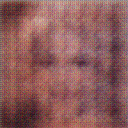
\includegraphics[width=150px]{500_fake_images/samples_5_194.png}%
\caption{A Black And White Photo Of A Zebra Standing In A Field}%
\end{figure}

%
\end{document}